\documentclass[journal,12pt,twocolumn]{IEEEtran}
\IEEEoverridecommandlockouts
\usepackage{cite}
\usepackage{amsmath,amssymb,amsfonts,bm}
\usepackage{mathtools}
\usepackage{tkz-euclide} 
\usetikzlibrary{calc,math}
 \usepackage{caption}
\usepackage{listings}
\let\vec\mathbf
\newcommand{\myvec}[1]{\ensuremath{\begin{pmatrix}#1\end{pmatrix}}}
\newcommand{\norm}[1]{\left\lVert#1\right\rVert}

\begin{document}

\title{Matrix Theory EE5609 - Assignment 3\\
Find if a triangle is isosceles triangle.
}

\author{\IEEEauthorblockN{Sandhya Addetla}\\
\IEEEauthorblockA{PhD Artificial Inteligence Department} \\
26-Sep-2020\\
AI20RESCH14001\\
 }

\maketitle
\begin{abstract}
This document provides a solution for finding if a traingle is isosceles given two equal altitudes of the triangle
\end{abstract}

\section{Problem Statement}
BE and CF are two equal altitudes of a triangle ABC. Prove that the triangle ABC is isosceles.


\section{Solution}
Given that BE and CF are two equal altitudes of a triangle ABC.

\captionsetup{justification=centering}

\begin{figure}[!h]
\centering
%\includegraphics[width=0.7\columnwidth]{
\resizebox{.5\columnwidth}{!}{
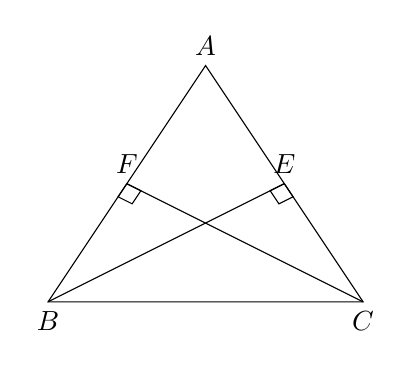
\begin{tikzpicture} 
        \coordinate (A) at (2, 3) {};
        \coordinate (B) at (0, 0) {};
        \coordinate (C) at (4, 0) {};
        \coordinate (F) at (1, 1.5) {};
        \coordinate (E) at (3, 1.5) {};
\draw (A)node[above]{$A$}--(B)node[below]{$B$}--(C)node[below]{$C$}--cycle;
\draw (B)node[below]{}--(E)node[above]{$E$};
\draw (C)node[below]{}--(F)node[above]{$F$};
\tkzMarkRightAngle[size=.2](B,E,C);
\tkzLabelAngle[dist=.5](B,E,C){};
\tkzMarkRightAngle[size=.2](C,F,B);
\tkzLabelAngle[dist=.5](C,F,B){};
\end{tikzpicture}
}
\caption{Triangle with equal altitudes on two sides}
\label{myfig}
\end{figure}
So, we have :-
 \begin{align}
 	\norm{\vec{E - B}} = \norm{\vec{F - C}} \label{1}
 \end{align}
Let $\textbf{m}_{AB}$ and $\textbf{m}_{CF}$ are the direction vectors of AB and CF respectively. Since AB $\perp$ CF hence,
\begin{align}
 \textbf{m}_{AB} \textbf{m}_{CF} = 0 \\
 \vec{\left( B - E\right)^T \left(A - C \right)} =\vec{ 0} \\
\vec{\left( B -  A + A - C + C - E\right)^T \left(A - C \right)} = \vec{0}
\end{align}
  \begin{multline} 
 \vec{ \left( B -  A \right)^T \left(A - C \right)} + \norm{\vec {A - C}}^{2} +\\ \vec{\left(C - F\right)^T \left(A - C \right)} = \vec{0} \label{5}
\end{multline} 

Similarly, AC $\perp$ BE hence,  
 \begin{align}
 \textbf{m}_{AC} \textbf{m}_{BE} = 0\\
 \vec{\left( C - F\right)^T \left(A - B \right)} =\vec{ 0} \\
 \vec{\left( C -  A + A - B + B - F\right)^T \left(A - B \right)} = \vec{0}
 \end{align}
 
  \begin{multline} 
 \vec{ \left( C-  A \right)^T \left(A - B \right)} + \norm{\vec {A - B}}^{2} + \\ \vec{\left(B - F\right)^T \left(A - B \right)} = \vec{0} \label{9}
  \end{multline} 
   
   In $\triangle ABC$, taking inner product of sides  AB and AC we can write :
   \begin{align}
\implies \cos \angle BAC = \frac{\left( \vec{ B - A} \right)^T  \left( \vec{A - C } \right)}{\norm{\vec{ B - A}} \norm{\vec{A - C}}} \label{11}
\end{align}  
Simlilarly,
 \begin{align}
  \cos \angle CAB = \frac{\left( \vec{C - A} \right)^T \left( \vec{A - B} \right) }{\norm{\vec{C - A}} \norm{\vec{ A - B}}}  \label{13}
\end{align}  
  
  From equation \ref{11}, and \ref{13}, we have ,
  \begin{multline} 
    \left( \vec{ B - A} \right)^T  \left( \vec{A - C } \right) =  \left( \vec{ C - A} \right)^T  \left( \vec{A - B } \right) \label{14}
   \end{multline} 
 using equation \ref{14} in \ref{5} and \ref{9} we can write,
   \begin{multline} 
   \norm{\vec{A - C}}^2 + \left ( \vec{ C - E }\right)^T \left( \vec{A - C} \right)  =  \\ \norm{\vec{A - B}}^2 + \vec{\left (  B - F\right)^{T} \left( A - B \right)}
    \end{multline} 
   
  \begin{multline} 
\norm{\vec{A - C}}^2 + \left ( \vec{ C - E }\right)^T \left( \vec{A - C} \right)  =  \\ \norm{\vec{A - B}}^2 + \vec{\left (  B - F\right)^{T} \left( A - B \right)}
 \end{multline}   
   
    \begin{multline} 
  \norm{\vec{A - C}}^2 +\\ \left ( \vec{ C - A + A - B +B - E }\right)^T \left( \vec{A - C} \right)  = \\ \norm{\vec{A - B}}^2 +\\ \vec{\left (  B - A + A - C + C - F\right)^{T} \left( A - B \right)}
   \end{multline}   
  
 \begin{multline} 
\norm{\vec{A - C}}^2 +  \norm{\vec{A - C}}^2 + \left ( \vec{  A - B  }\right)^T \left( \vec{A - C} \right) +\\ \left ( \vec{   B - E }\right)^T  \left( \vec{A - C} \right) =   \norm{\vec{A - B}}^2 +\\ \norm{\vec{A - B}}^2 + \vec{\left ( A - C \right)^{T} \left( A - B \right)}  + \\ \vec{\left (  C - F\right)^{T} \left( A - B \right)} \label{18}
 \end{multline}    
  
since BE $\perp$ AC and CF $\perp$ AB, hence :
\begin{align}
 \left ( \vec{   B - E }\right)^T \left( \vec{A - C} \right) = \vec{0} \\
  \vec{\left (  C - F\right)^{T} \left( A - B \right)} = \vec{0}
\end{align}
Now equation \ref{18} become :
 \begin{multline}
2\norm{\vec{A - C}}^2 + \left ( \vec{  A - B  }\right)^T \left( \vec{A - C} \right)    =  \\ 2 \norm{\vec{A - B}}^2 + \vec{\left ( A - C \right)^{T} \left( A - B \right)} \label{21}
 \end{multline} 
  Substituting equation \ref{14} in equation \ref{21},
    \begin{align}
  \norm{\vec{A - C} } = \norm {\vec{A - B}}
  \end{align}
  Therefore,  the magnitude of sides AB and AC of $\triangle ABC$ are equal and hence they form the sides of an isosceles triangle.
\end{document}